\documentclass[14pt]{extbook}
\usepackage{multicol, enumerate, enumitem, hyperref, color, soul, setspace, parskip, fancyhdr} %General Packages
\usepackage{amssymb, amsthm, amsmath, latexsym, units, mathtools} %Math Packages
\everymath{\displaystyle} %All math in Display Style
% Packages with additional options
\usepackage[headsep=0.5cm,headheight=12pt, left=1 in,right= 1 in,top= 1 in,bottom= 1 in]{geometry}
\usepackage[usenames,dvipsnames]{xcolor}
\usepackage{dashrule}  % Package to use the command below to create lines between items
\newcommand{\litem}[1]{\item#1\hspace*{-1cm}\rule{\textwidth}{0.4pt}}
\pagestyle{fancy}
\lhead{Progress Quiz 6}
\chead{}
\rhead{Version C}
\lfoot{1430-1829}
\cfoot{}
\rfoot{test}
\begin{document}

\begin{enumerate}
\litem{
Write the equation of the graph presented below in the form $f(x)=ax^2+bx+c$, assuming  $a=1$ or $a=-1$. Then, choose the intervals that $a, b,$ and $c$ belong to.
\begin{center}
    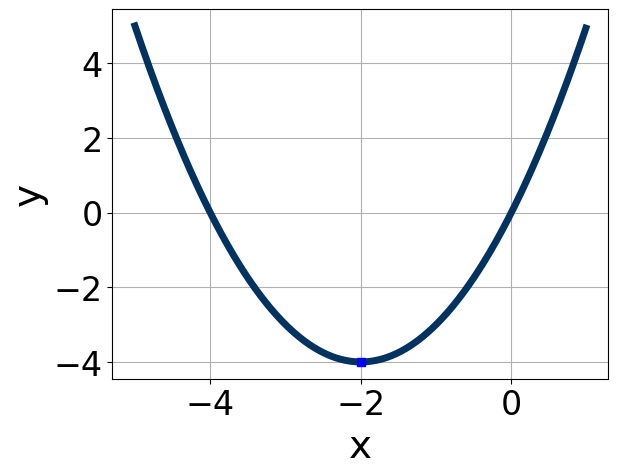
\includegraphics[width=0.5\textwidth]{../Figures/quadraticGraphToEquationCopyC.png}
\end{center}
\begin{enumerate}[label=\Alph*.]
\item \( a \in [0, 1.9], \hspace*{5mm} b \in [0, 9], \text{ and } \hspace*{5mm} c \in [10, 11] \)
\item \( a \in [0, 1.9], \hspace*{5mm} b \in [-7, -3], \text{ and } \hspace*{5mm} c \in [-2, 2] \)
\item \( a \in [0, 1.9], \hspace*{5mm} b \in [0, 9], \text{ and } \hspace*{5mm} c \in [-2, 2] \)
\item \( a \in [-2.3, -0.6], \hspace*{5mm} b \in [0, 9], \text{ and } \hspace*{5mm} c \in [-12, -9] \)
\item \( a \in [-2.3, -0.6], \hspace*{5mm} b \in [-7, -3], \text{ and } \hspace*{5mm} c \in [-12, -9] \)

\end{enumerate} }
\litem{
Factor the quadratic below. Then, choose the intervals that contain the constants in the form $(ax+b)(cx+d); b \leq d.$\[ 24x^{2} +50 x + 25 \]\begin{enumerate}[label=\Alph*.]
\item \( a \in [3.59, 5.5], \hspace*{5mm} b \in [4, 11], \hspace*{5mm} c \in [5.91, 6.34], \text{ and } \hspace*{5mm} d \in [1, 6] \)
\item \( a \in [1.68, 3.64], \hspace*{5mm} b \in [4, 11], \hspace*{5mm} c \in [11.87, 12.15], \text{ and } \hspace*{5mm} d \in [1, 6] \)
\item \( a \in [-1.04, 1.56], \hspace*{5mm} b \in [17, 26], \hspace*{5mm} c \in [0.92, 1.21], \text{ and } \hspace*{5mm} d \in [23, 33] \)
\item \( a \in [11.73, 13.03], \hspace*{5mm} b \in [4, 11], \hspace*{5mm} c \in [1.2, 2.99], \text{ and } \hspace*{5mm} d \in [1, 6] \)
\item \( \text{None of the above.} \)

\end{enumerate} }
\litem{
Solve the quadratic equation below. Then, choose the intervals that the solutions $x_1$ and $x_2$ belong to, with $x_1 \leq x_2$.\[ 15x^{2} +2 x -24 = 0 \]\begin{enumerate}[label=\Alph*.]
\item \( x_1 \in [-0.84, 0.34] \text{ and } x_2 \in [2.23, 2.89] \)
\item \( x_1 \in [-20.64, -19.82] \text{ and } x_2 \in [17.81, 18.57] \)
\item \( x_1 \in [-2.86, -1.67] \text{ and } x_2 \in [0.52, 0.81] \)
\item \( x_1 \in [-4.09, -3.97] \text{ and } x_2 \in [0.35, 0.45] \)
\item \( x_1 \in [-1.46, -0.8] \text{ and } x_2 \in [1.17, 1.62] \)

\end{enumerate} }
\litem{
Graph the equation below.\[ f(x) = (x+2)^2 + 13 \]\begin{enumerate}[label=\Alph*.]
\begin{multicols}{2}\item 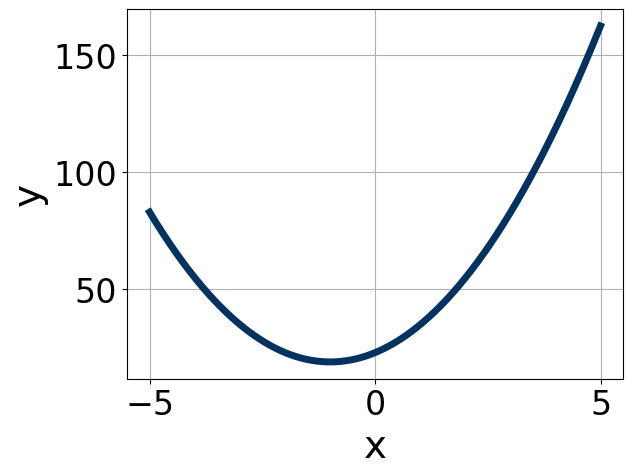
\includegraphics[width = 0.3\textwidth]{../Figures/quadraticEquationToGraphCopyAC.png}\item 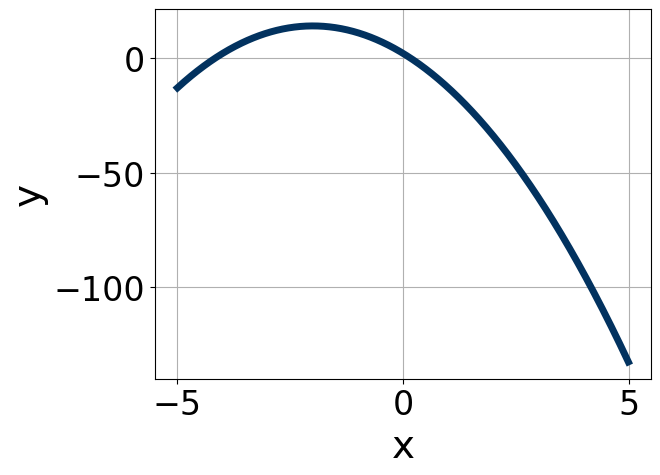
\includegraphics[width = 0.3\textwidth]{../Figures/quadraticEquationToGraphCopyBC.png}\item 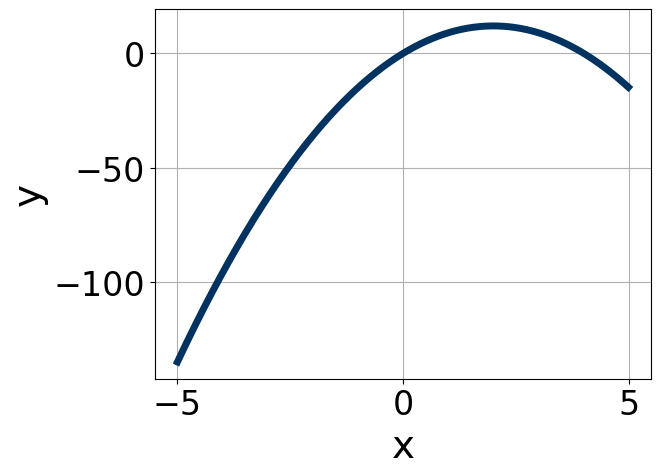
\includegraphics[width = 0.3\textwidth]{../Figures/quadraticEquationToGraphCopyCC.png}\item 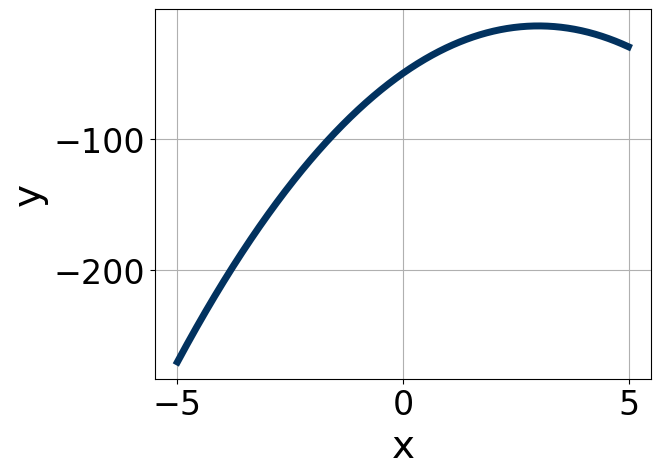
\includegraphics[width = 0.3\textwidth]{../Figures/quadraticEquationToGraphCopyDC.png}\end{multicols}\item None of the above.
\end{enumerate} }
\litem{
Graph the equation below.\[ f(x) = (x-1)^2 - 10 \]\begin{enumerate}[label=\Alph*.]
\begin{multicols}{2}\item 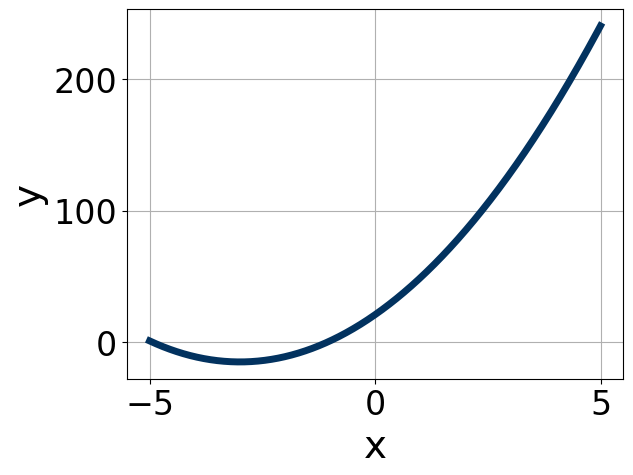
\includegraphics[width = 0.3\textwidth]{../Figures/quadraticEquationToGraphAC.png}\item 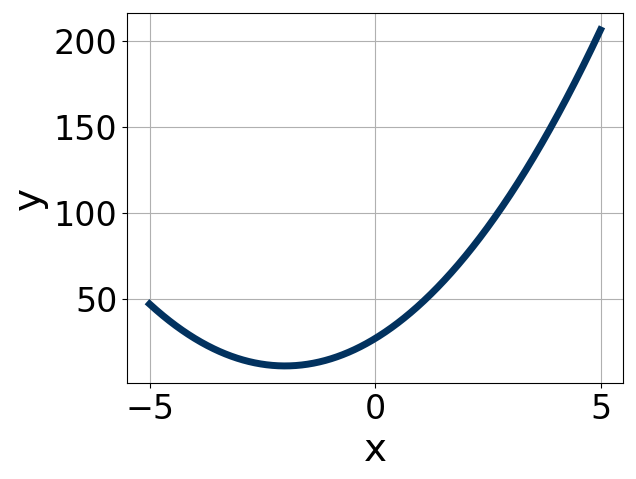
\includegraphics[width = 0.3\textwidth]{../Figures/quadraticEquationToGraphBC.png}\item 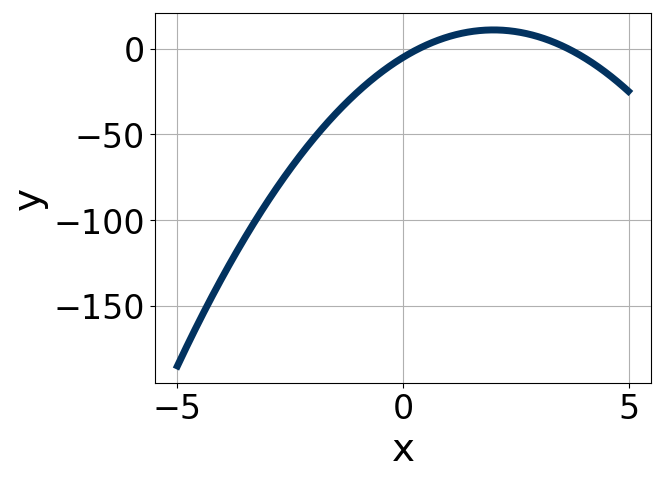
\includegraphics[width = 0.3\textwidth]{../Figures/quadraticEquationToGraphCC.png}\item 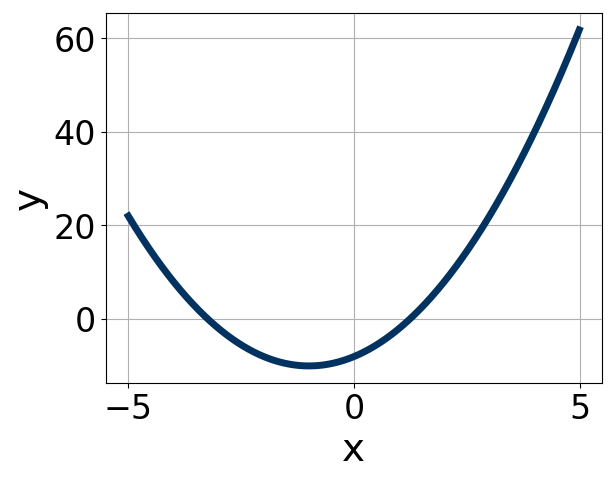
\includegraphics[width = 0.3\textwidth]{../Figures/quadraticEquationToGraphDC.png}\end{multicols}\item None of the above.
\end{enumerate} }
\litem{
Write the equation of the graph presented below in the form $f(x)=ax^2+bx+c$, assuming  $a=1$ or $a=-1$. Then, choose the intervals that $a, b,$ and $c$ belong to.
\begin{center}
    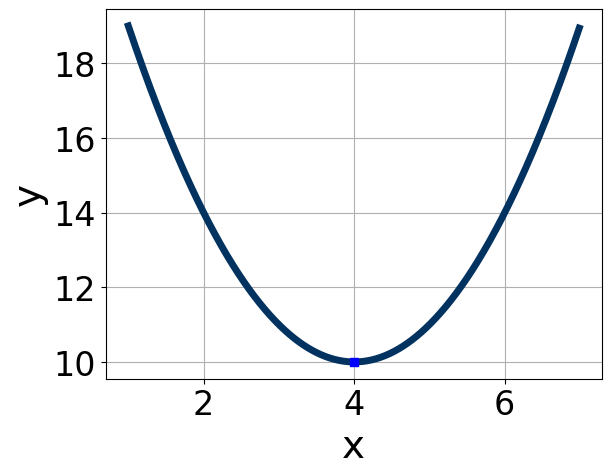
\includegraphics[width=0.5\textwidth]{../Figures/quadraticGraphToEquationC.png}
\end{center}
\begin{enumerate}[label=\Alph*.]
\item \( a \in [1, 5], \hspace*{5mm} b \in [-9, -7], \text{ and } \hspace*{5mm} c \in [9, 14] \)
\item \( a \in [1, 5], \hspace*{5mm} b \in [6, 12], \text{ and } \hspace*{5mm} c \in [9, 14] \)
\item \( a \in [-3, 0], \hspace*{5mm} b \in [-9, -7], \text{ and } \hspace*{5mm} c \in [-13, -11] \)
\item \( a \in [-3, 0], \hspace*{5mm} b \in [-9, -7], \text{ and } \hspace*{5mm} c \in [-22, -19] \)
\item \( a \in [-3, 0], \hspace*{5mm} b \in [6, 12], \text{ and } \hspace*{5mm} c \in [-22, -19] \)

\end{enumerate} }
\litem{
Solve the quadratic equation below. Then, choose the intervals that the solutions $x_1$ and $x_2$ belong to, with $x_1 \leq x_2$.\[ 25x^{2} -60 x + 36 = 0 \]\begin{enumerate}[label=\Alph*.]
\item \( x_1 \in [1.2, 1.28] \text{ and } x_2 \in [0.02, 2.18] \)
\item \( x_1 \in [29.84, 30.02] \text{ and } x_2 \in [29.27, 30.72] \)
\item \( x_1 \in [0.51, 0.68] \text{ and } x_2 \in [2.07, 2.53] \)
\item \( x_1 \in [0.22, 0.28] \text{ and } x_2 \in [5.71, 6.33] \)
\item \( x_1 \in [0.32, 0.41] \text{ and } x_2 \in [2.97, 4.3] \)

\end{enumerate} }
\litem{
Factor the quadratic below. Then, choose the intervals that contain the constants in the form $(ax+b)(cx+d); b \leq d.$\[ 36x^{2} +43 x + 12 \]\begin{enumerate}[label=\Alph*.]
\item \( a \in [-0.7, 1.2], \hspace*{5mm} b \in [15, 19], \hspace*{5mm} c \in [-4.7, 3.3], \text{ and } \hspace*{5mm} d \in [23, 28] \)
\item \( a \in [-0.7, 1.2], \hspace*{5mm} b \in [-3, 10], \hspace*{5mm} c \in [24.8, 30.7], \text{ and } \hspace*{5mm} d \in [0, 7] \)
\item \( a \in [5.6, 10.6], \hspace*{5mm} b \in [-3, 10], \hspace*{5mm} c \in [3.3, 5.9], \text{ and } \hspace*{5mm} d \in [0, 7] \)
\item \( a \in [2.1, 5.6], \hspace*{5mm} b \in [-3, 10], \hspace*{5mm} c \in [8.8, 10.7], \text{ and } \hspace*{5mm} d \in [0, 7] \)
\item \( \text{None of the above.} \)

\end{enumerate} }
\litem{
Solve the quadratic equation below. Then, choose the intervals that the solutions belong to, with $x_1 \leq x_2$ (if they exist).\[ 16x^{2} +13 x -6 = 0 \]\begin{enumerate}[label=\Alph*.]
\item \( x_1 \in [-21.2, -17.8] \text{ and } x_2 \in [5, 6.1] \)
\item \( x_1 \in [-25.3, -23.6] \text{ and } x_2 \in [22.2, 25.4] \)
\item \( x_1 \in [-1.1, 1] \text{ and } x_2 \in [0.6, 2.2] \)
\item \( x_1 \in [-1.3, -0.6] \text{ and } x_2 \in [-0.1, 0.4] \)
\item \( \text{There are no Real solutions.} \)

\end{enumerate} }
\litem{
Solve the quadratic equation below. Then, choose the intervals that the solutions belong to, with $x_1 \leq x_2$ (if they exist).\[ -11x^{2} +7 x + 6 = 0 \]\begin{enumerate}[label=\Alph*.]
\item \( x_1 \in [-17.74, -16.31] \text{ and } x_2 \in [17.57, 18.71] \)
\item \( x_1 \in [-12.67, -12.24] \text{ and } x_2 \in [5.23, 5.44] \)
\item \( x_1 \in [-1.02, 0.29] \text{ and } x_2 \in [0.74, 1.56] \)
\item \( x_1 \in [-1.8, -0.97] \text{ and } x_2 \in [-0.29, 0.66] \)
\item \( \text{There are no Real solutions.} \)

\end{enumerate} }
\end{enumerate}

\end{document}